\chapter{PENGENALAN SOFTWARE}

\begin{enumerate}[\bfseries A.]

  \item \textbf{Membuka Program}
  
  \begin{enumerate}[1.]
  
    \item Pilih Start -\textgreater Program -\textgreater MapInfo -\textgreater MapInfo 8. Muncul tampilan jendela berikut :
    
    \begin{figure}[H]
      \centering
      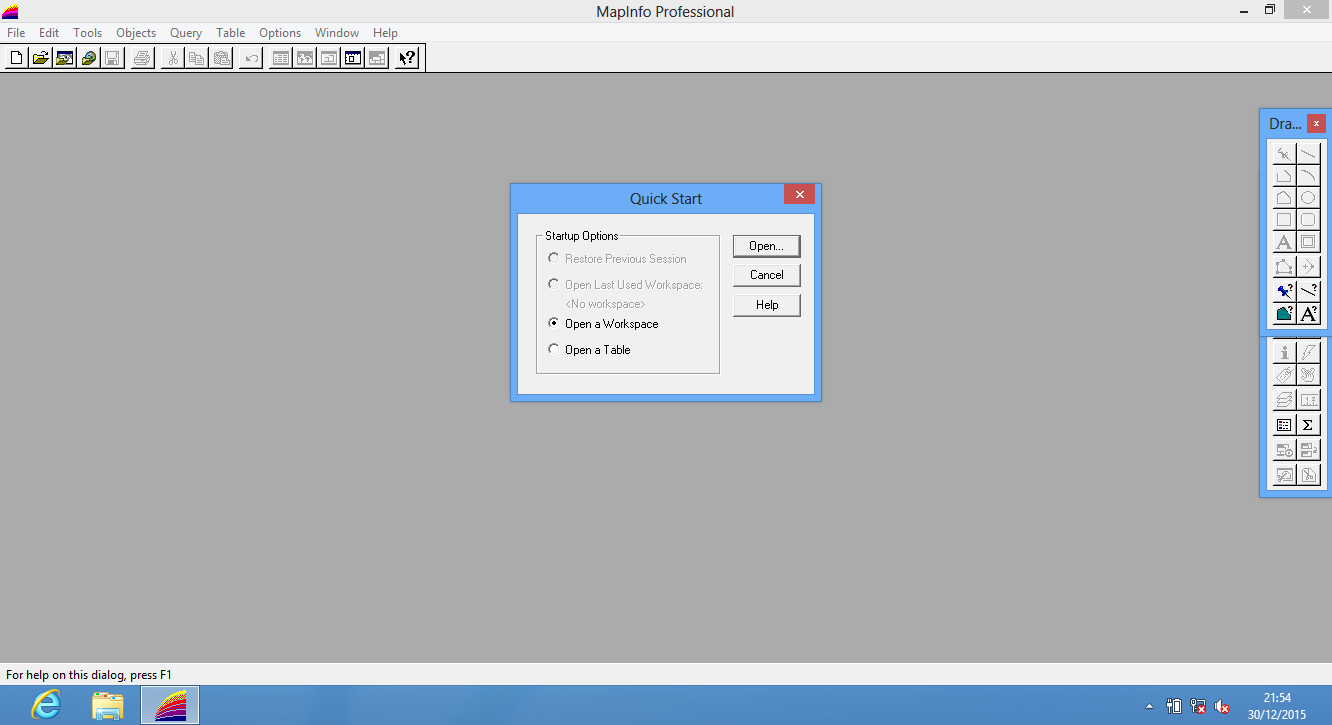
\includegraphics[width=1\textwidth]{./resources/000-start-mapinfo8}
      \caption{Jendela awal Mapinfo 8}
    \end{figure}
    
    \item Klik \textbf{Cancel} pada box \textit{Quick Start}
    
    \item Drag box \textbf{Main} dan \textbf{Standard} ke atas, tempatkan dibawah menu utama, menjadi seperti tampilan berikut :
  
    \begin{figure}[H]  
      \centering
      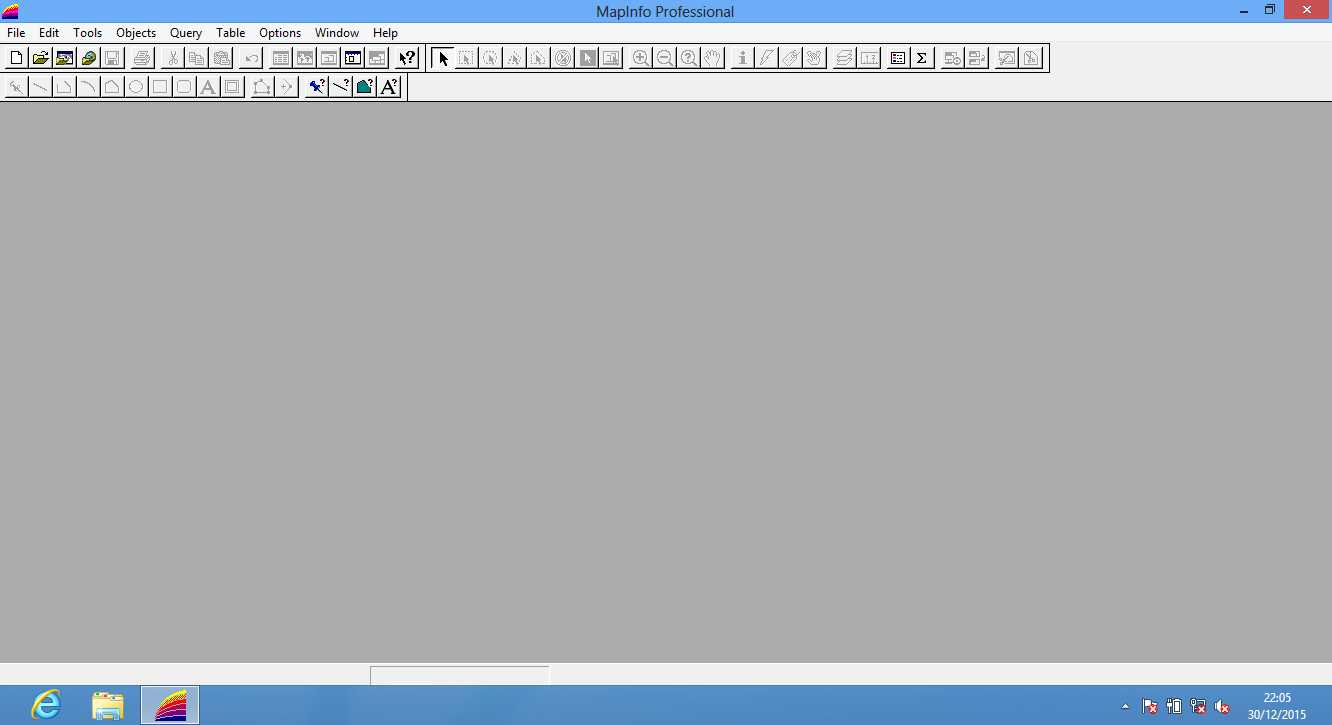
\includegraphics[width=1\textwidth]{./resources/001-rapih-icon}
      \caption{Posisi Icon Yang Telah Dirapihkan}
    \end{figure}
  
  \end{enumerate}
  
  \item \textbf{Membuat File Baru}
  
  \begin{enumerate}[1.]
  
    \item Pilih File -\textgreater New Table, sehingga muncul tampilan berikut :
    
    \begin{figure}[H]
      \centering
      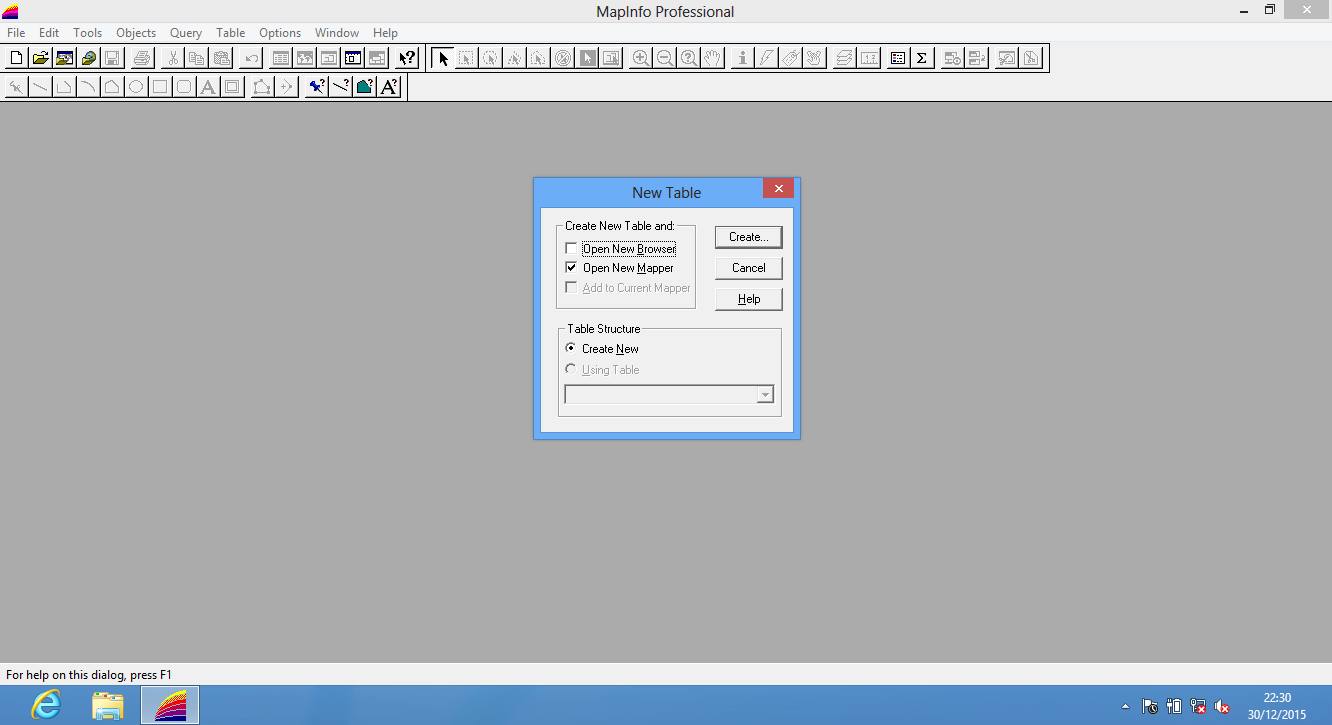
\includegraphics[width=1\textwidth]{./resources/002-new-mapper}
      \caption{Jendela Membuat File Baru}
    \end{figure}
    
    \item Kemudian tekan tombol \textbf{Create} sehingga muncul jendela berikut :
    
    \begin{figure}[H]
      \centering
	  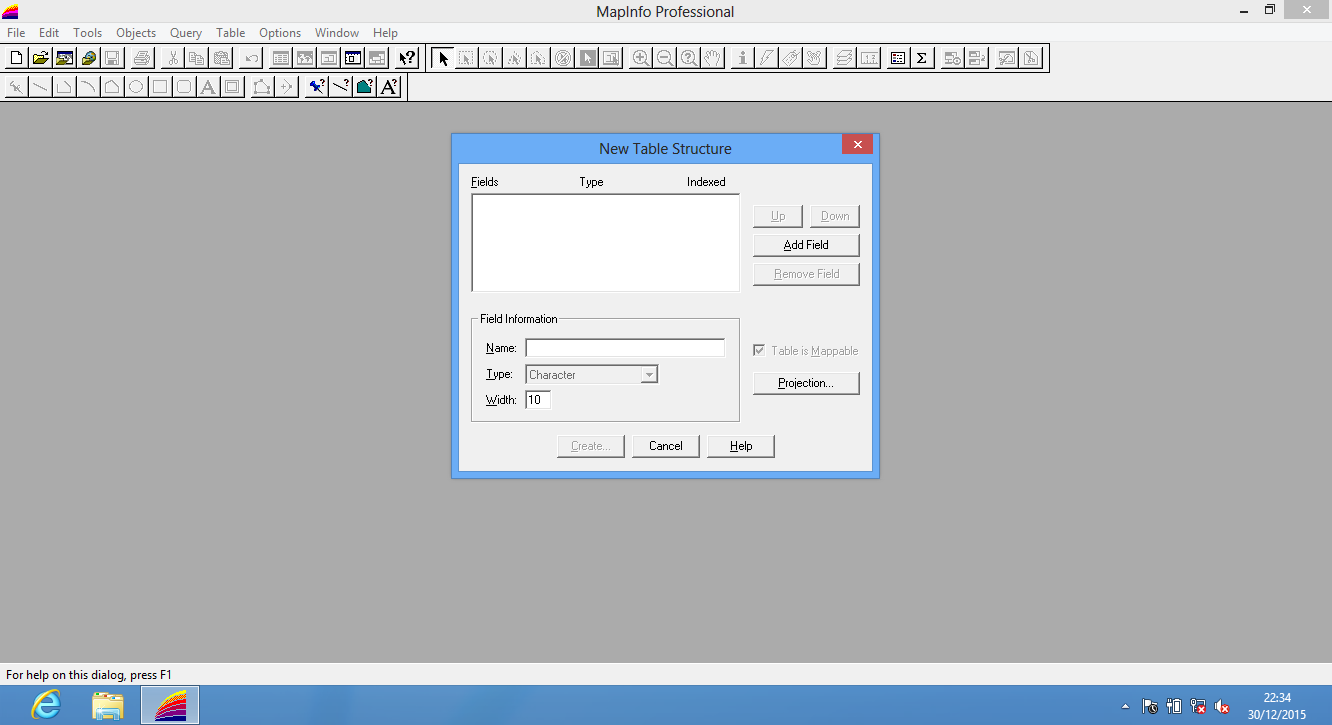
\includegraphics[width=1\textwidth]{./resources/003-pembentukan-tabel}
	  \caption{Jendela pembentukan field tabel}
	\end{figure}
    
    \item Untuk pengisian nama field, nantinya akan disesuaikan dengan jenis layer yang akan kita bangun. Sebagai contoh, apabila nanti akan membuat layer bidang, akan ada field d\_nop untuk menyimpan NOP bidangnya, apabila nanti akan membuat layer jalan, maka akan ada field d\_nm\_jln untuk menyimpan nama jalan.
    
    Sebagai referensi pembuatan field-field apa saja yang dibentuk sesuai dengan kondisi layernya, maka berikut disajikan aturan penamaan field sesuai dengan Peraturan Bupati Brebes tentang Pedoman Pendaftaran, Pendataan, Penilaian, dan Pelaporan Objek dan Subjek Pajak Bumi dan Bangunan Perdesaan dan Perkotaan di Kabupaten Brebes.
    
    \begin{enumerate}[1.]
    
      \item Layer Tanah/Bidang
      
        Layer ini berisi tanah/bidang objek pajak dalam satu Desa/Kelurahan, dimana penamaan \textit{file} mengikuti aturan 3329KKKLLL, dimana \textbf{KKK} berisi 3 (tiga) digit kode Kecamatan, dan \textbf{LLL} berisi 3 (tiga) digit kode Kelurahan/Desa.
      
        Gambar memiliki tipe \textbf{poligon}, dengan \textit{Fill Pattern} \textbf{none}, \textit{Border Style} \textbf{Garis penuh}, \textit{Color} \textbf{Black}, \textit{width} \textbf{0,17mm}
        
        \textit{Struktur basis data}
      
        \begin{tabular}{| l | c | c | p{5cm} |}
          \hline
          Nama Field & Type & Index & Keterangan \\
          \hline
          d\_nop & character(18) & index 1 & NOP setiap bidang tanah \\
          \hline
          d\_luas & decimal(10,2) & & Luas Bidang tanah dengan menggunakan update  column terhadap field \textbf{d\_luas} dengan value assist function area. \\
          \hline          
        \end{tabular}
        
      \item Layer Bangunan
      
        Layer ini berisi gambar denah bangunan dalam satu Desa/Kelurahan, dimana penamaan \textit{file} mengikuti aturan 3329KKKLLLbg, dimana \textbf{KKK} berisi 3 (tiga) digit kode Kecamatan, dan \textbf{LLL} berisi 3 (tiga) digit kode Kelurahan/Desa.
      
        Gambar memiliki tipe \textbf{poligon}, \textit{Fill Pattern} \textbf{(MapInfo No. 5)}, \textit{Foreground} \textbf{(MapInfo no. 7)}, \textit{Background} \textbf{none}, \textit{Border Style} \textbf{Garis Putus} (\textit{line style} \textbf{MapInfo No. 5}, \textit{Color} \textbf{Hijau}, \textit{width} \textbf{0,17mm}
        
        \textit{Struktur basis data}
      
        \begin{tabular}{| l | c | c | p{5cm} |}
          \hline
          Nama Field & Type & Index & Keterangan \\
          \hline
          d\_nop & character(21) & Index 1 & NOP ditambah nomor bangunan setiap bangunannya.\\
          \hline
        \end{tabular}
      
      \item Layer Jalan
      
        Layer ini berisi gambar jalan dalam satu Desa/Kelurahan, dimana penamaan \textit{file} untuk layer ini mengikuti aturan 3329KKKLLLjl, dimana \textbf{KKK} berisi 3 (tiga) digit kode Kecamatan, dan \textbf{LLL} berisi 3 (tiga) digit kode Kelurahan/Desa.
      
        Gambar memiliki tipe \textbf{Polyline}, \textit{Style} \textbf{Garis Penuh}, \textit{color} \textbf{red}, \textit{width} \textbf{0,17mm}
        
        \textit{Struktur basis data}
      
        \begin{tabular}{| l | c | c | p{5cm} |}
          \hline
          Nama Field & Type & Index & Keterangan \\
          \hline
          d\_nm\_jln & character(30) & & Nama Jalan \\
          \hline
          d\_lbr\_jln & Integer & & Lebar jalan (rata-rata lebar pada jalan tersebut) \\    
          \hline
        \end{tabular}

      
      \item Layer Sungai
      
        Layer ini berisi gambar sungai dalam satu Desa/Kelurahan, dimana penamaan \textit{file} untuk layer ini mengikuti aturan 3329KKKLLLsg, dimana \textbf{KKK} berisi 3 (tiga) digit kode Kecamatan, dan \textbf{LLL} berisi 3 (tiga) digit kode Kelurahan/Desa.
      
        Gambar memiliki tipe \textbf{polyline}, \textit{style} \textbf{Garis penuh}, \textit{color} \textbf{blue}, \textit{width} \textbf{0,17mm}
        
        \textit{Struktur basis data}
      
        \begin{tabular}{| l | c | c | p{5cm} |}
          \hline
          Nama Field & Type & Index & Keterangan \\
          \hline
          d\_nm\_sng & character(30) &  & Nama Sungai \\
          \hline
          d\_lbr\_sng & integer & & Lebar sungai (rata-rata lebar pada sungai tersebut) \\
          \hline
        \end{tabular}
      
      \item Layer Text
      
        Layer ini berisi keterangan teks dalam satu Desa/Kelurahan, penamaan \textit{file} untuk layer ini mengikuti aturan 3329KKKLLLtx, dimana \textbf{KKK} berisi 3 (tiga) digit kode Kecamatan, dan \textbf{LLL} berisi 3 (tiga) digit kode Kelurahan/Desa.
      
        \begin{tabular}{| l | c | c | p{5cm} |}
          \hline
          Nama Field & Type & Index & Keterangan \\
          \hline
          d\_text & character(30) & & Sebagai penjelas / keterangan pada bidang cetak peta \\
          \hline
        \end{tabular}
        
        kolom d\_text dapat berisi :
        
        \begin{itemize}
          \item Teks mengenai keseluruhan nama utilitas jalan, sungai, informasi nama wilayah yang bersebelahan, informasi lokasi penting, dan sebagainya, yang tidak terdapat termasuk layer-layer lain berwarna hitam dengan tipe huruf \textit{italic} berukuran sesuai dengan gambar.
          \item Batas tepi jalan diperkeras berwarna merah ukuran garis paling tipis
          \item Batas tepi jalan tidak diperkeras berwarna coklat kekuningan berukuran garis paling tipis.
          \item Batas tepi jalan TOL berwarna merah berukuran garis tipis no. 2,
          \item Batas tepi sungai berwarna biru berukuran garis tipis no.2
          \item Utilitas yang disertai dengan simbolnya.
        \end{itemize}
      
      \item Layer Batas Blok
      
        Layer ini menggambarkan batas blok dalam suatu Desa/Kelurahan, penamaan \textit{file} mengikuti aturan 3329KKKLLLbl, dimana \textbf{KKK} berisi 3 (tiga) digit kode Kecamatan, dan \textbf{LLL} berisi 3 (tiga) digit kode Kelurahan/Desa.
      
        Gambar memiliki \textit{tipe} \textbf{Polygon}, \textit{fill pattern} \textbf{None}, \textit{border style} \textbf{garis putus dan titik} (\textit{line style} \textbf{Mapinfo Nomor 13}, \textit{color} \textbf{blue}, \textit{width} \textbf{0,25mm}.
        
        \textit{Struktur Basis Data}
        
        \begin{tabular}{| l | c | c | p{5cm} |}
          \hline
          Nama Field & Type & Index & Keterangan \\
          \hline
          d\_blok & character(13) & & Kode wilayah + Nomor Blok \\
          \hline
        \end{tabular}
      
      \item Layer Simbol
      
      Layer ini digunakan untuk memberikan simbol simbol umum pada peta dalam satu Desa/Kelurahan. Penamaan \textit{file} untuk layer ini mengikuti aturan 3329KKKLLLsi, dimana \textbf{KKK} berisi 3 (tiga) digit kode Kecamatan, dan \textbf{LLL} berisi 3 (tiga) digit kode Desa/Kelurahan.
      
      \textit{Struktur Basis Data}
      
      \begin{tabular}{| l | c | c | p{5cm} |}
        \hline
        Nama Field & Type & Index & Keterangan \\
        \hline
        d\_kd\_simbol & character(4) & & Kode simbol \\
        \hline
      \end{tabular}
      
      \textit{Rincian Layer Simbol}
      
      \begin{tabular}{| c | c |}
        \hline
        Kode Simbol & Uraian Simbol \\
        \hline
        1 & Kuburan Islam \\
        \hline
        2 & Kuburan Kristen \\
        \hline
        3 & Kuburan Lainnya \\
        \hline
        4 & Masjid \\
        \hline
        5 & Gereja \\
        \hline
        6 & Candi \\
        \hline
        7 & Pura/Puri \\
        \hline
        8 & Klenteng \\
        \hline
        9 & Kantor \\
        \hline
        10 & Titik Triangulasi \\
        \hline
        11 & Tugu / Titik Poligon \\
        \hline
      \end{tabular}
      
      \item Layer Batas Kelurahan
      
      Layer ini berisi gambar batas wilayah administrasi tiap Desa/Kelurahan dalam satu Kecamatan. Penamaan \textit{file} untuk layer ini mengikuti aturan 3329KKK, dimana \textbf{KKK} berisi 3 (tiga) digit kode Kecamatan.
      
      Gambar memiliki \textit{tipe} \textbf{Polygon}, \textit{fill pattern} \textbf{none}, \textit{border style} \textbf{garis putus} (\textit{line style} \textbf{MapInfo Nomor 7}), \textit{color} \textbf{black}, \textit{width} \textbf{1 mm}.
      
      \textit{Struktur basis data} 
      
      \begin{tabular}{| l | c | c | p{5cm} |}
        \hline
        Nama Field & Type & Index & Keterangan \\
        \hline
        d\_kd\_kel & character(10) & & Kode wilayah Kelurahan \\
        \hline
        d\_nm\_kel & character(25) & & Nama Kelurahan \\
        \hline
      \end{tabular}
      
      \item Layer Batas Kecamatan
      
      Layer ini berisi gambar batas administrasi untuk tiap Kecamatan dalam 1 (satu) Kabupaten/Kota. Penamaan \textit{file} untuk layer ini hanya 3329, karena gambarnya hanya berisi batas administrasi Kecamatan di Kabupaten Brebes.
      
      Gambar memiliki \textit{tipe} \textbf{Polygon}, \textit{fill pattern} \textbf{none}, \textit{border style} \textbf{garis putus} (\textit{line style} \textbf{MapInfo Nomor 7}), \textit{color} \textbf{black}, \textit{width} \textbf{1 mm}.
      
      \textit{Struktur basis data}
      
      \begin{tabular}{| l | c | c | p{5cm} | }
        \hline
        Nama Field & Type & Index & Keterangan \\
        \hline
        d\_kd\_kec & character(7) & & Kode wilayah Kecamatan \\
        \hline
        d\_nm\_kec & character(25) & & Nama Kecamatan \\
        \hline
      \end{tabular}
      
      \item Layer Batas Kabupaten
      
      Layer ini berisi gambar batas administrasi Kabupaten, karena wilayah yang dibutuhkan hanya Kabupaten Brebes, maka hanya ada 1 (satu) \textit{file} untuk layer ini dengan nama \textit{file} diisikan 33.
      
      Gambar memiliki \textit{tipe} \textbf{polygon}, \textit{fill pattern} \textbf{none}, \textit{border style} \textbf{garis positif} (\textit{line style} \textbf{MapInfo nomor 32}), \textit{color} \textbf{black}, \textit{width} \textbf{1 mm}.
      
      \textit{Struktur basis data}
      
      \begin{tabular}{| l | c | c | p{5cm} |}
        \hline
        Nama Field & Type & Index & Keterangan \\
        \hline
        d\_kd\_dt2 & character(4) & & Kode wilayah Daerah Kabupaten \\
        \hline
        d\_nm\_dt2 & character(25) & & Nama Daerah Kabupaten \\
        \hline
      \end{tabular}
      
    \end{enumerate}
  
  \end{enumerate}
  
  \item \textbf{Membuat Layer}
  
  \begin{enumerate}[1.]
    \item Membuat \textit{workspace} baru atau membuka \textit{file} yang sudah ada.
  
    \item Pilih Map -\textgreater  Layer Control, atau cukup meng-klik ikon 
\includegraphics{./resources/004-ikon-layer-kontrol} . Sehingga akan tampil jendela berikut :
    
    \begin{figure}[H]
      \centering
      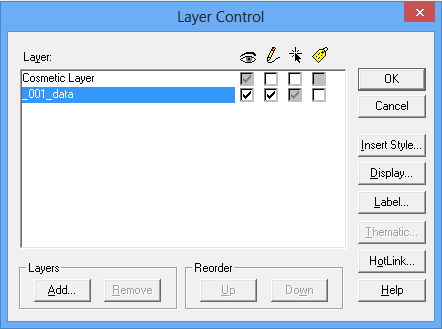
\includegraphics[width=1\textwidth]{./resources/005-jendela-layer-control}
      \caption{Jendela Layer Control}
    \end{figure}
    
    \item Pastikan bahwa file ini sudah dalam kondisi dapat di-edit. Lalu pilih \textbf{OK}. Ciri-ciri bahwa layer ini sudah dapat di-edit dapat dilihat tanda centang pada gambar berikut :
    
    \begin{figure}[H]
      \centering
      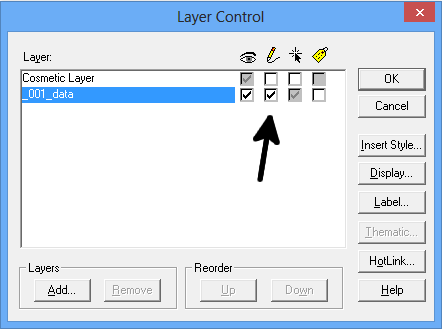
\includegraphics[width=1\textwidth]{./resources/006-mode-edited}
      \caption{Layer Dapat Diedit\label{fig:layeredited}}
    \end{figure}
    
    \item Buat objek titik, garis, atau polygon dengan meng-klik ikon-ikon berikut :
    
    \begin{figure}[H]
      \centering
      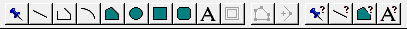
\includegraphics[width=1\textwidth]{./resources/007-ikon-drawing}
      \caption{Ikon Untuk Membuat Objek}
    \end{figure}
    
    \item Jika selesai, simpan dengan memilih menu File -\textgreater Save Table -\textgreater Save. 
  \end{enumerate}
  
  \item \textbf{Mengedit File}
  
  \begin{enumerate}[1.]
    \item Buka \textit{file} yang sudah dibuat, atau buat layer baru, lalu pastikan \textit{file} dalam kondisi dapat di-edit dengan meng-klik Map -\textgreater Layer Control sehingga tampil jendela seperti gambar \ref{fig:layeredited}
    
    \item Pilih objek yang akan di edit dengan meng-klik ikon \textbf{select} seperti ini 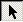
\includegraphics{./resources/008-ikon-select}
    
    \item Pilih ikon Reshape untuk menampilkan vertex, yang berbentuk seperti ini 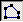
\includegraphics{./resources/009-ikon-reshape} klik salah satu vertex lalu tarik ke arah lain.
    
    Sebagai contoh, bentuk objek yang akan kita ubah dengan fungsi \textit{reshape} adalah seperti ini :
    
    \begin{figure}[H]
      \centering
      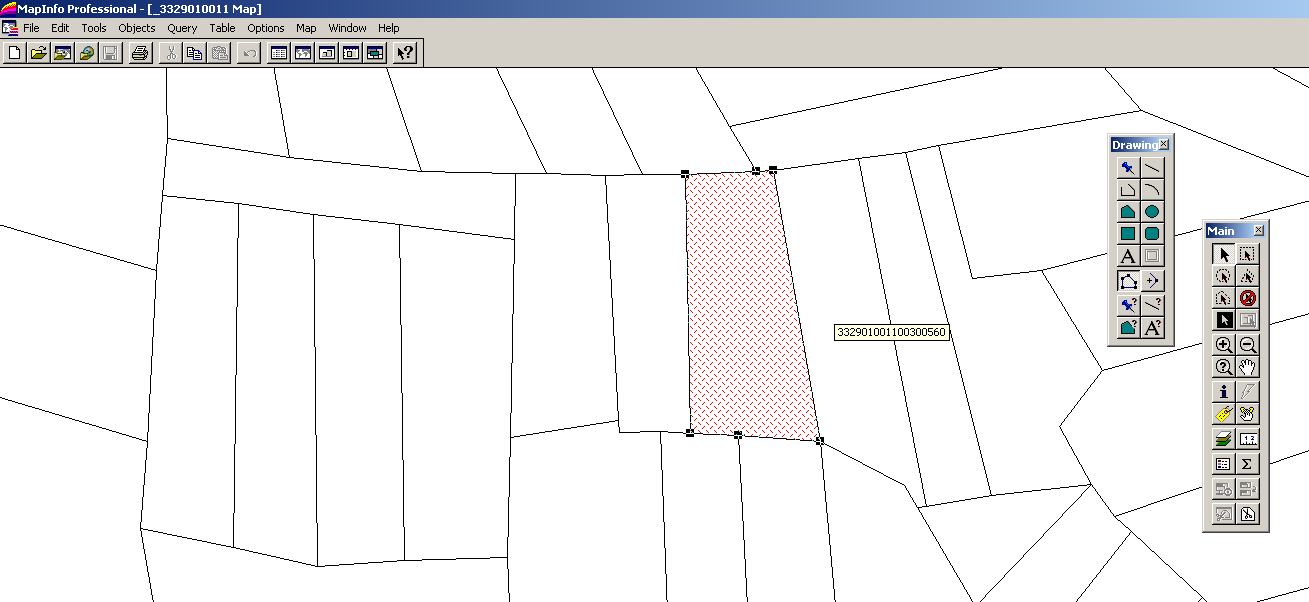
\includegraphics[width=1\textwidth]{./resources/010-sebelum-reshape}
      \caption{Bentuk Bidang Sebelum dilakukan Reshape}
    \end{figure}
    
    Dan contoh bentuk objek setelah kita ubah dengan fungsi \textit{reshape} menjadi seperti ini :
    
    \begin{figure}[H]
      \centering
      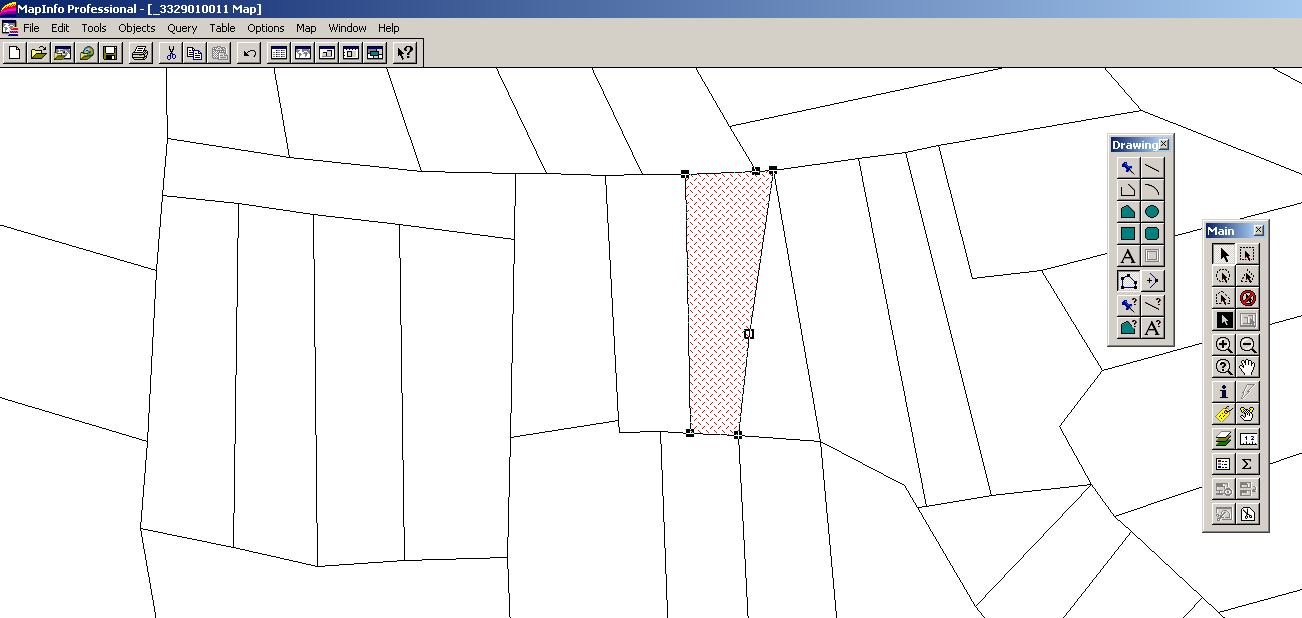
\includegraphics[width=1\textwidth]{./resources/011-sesudah-reshape}
      \caption{Bentuk Bidang Setelah dilakukan Reshape}
    \end{figure}
    
    \item Pilih ikon Add Node untuk menambah vertex. Bentuk ikonnya seperti ini 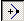
\includegraphics{./resources/012-ikon-add-node}
  \end{enumerate}
  
  \item \textbf{Operasi Penggabungan (Combine)}
  
  \begin{enumerate}[1.]
    \item Bukalah terlebih dahulu layer yang akan digabungkan objeknya, atau buat baru layer dengan dua objek yang akan digabungkan. Sebagai contoh seperti gambar berikut :
    
    \begin{figure}[H]
      \centering
      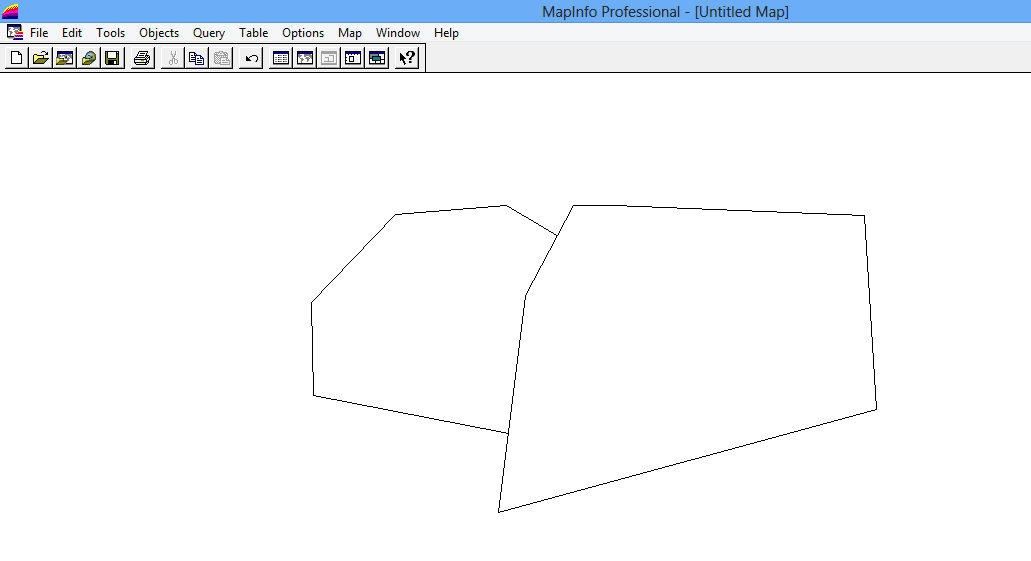
\includegraphics[width=1\textwidth]{./resources/013-layer-untuk-combine}
      \caption{Contoh Bentuk Bidang-Bidang Yang Akan Digabungkan}
    \end{figure}
    
    \item Pilih dua objek yang akan digabung dengan menggunakan ikon \textit{select} seperti ini 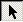
\includegraphics{./resources/008-ikon-select} dengan menekan tombol Shift pada \textit{keyboard}, sehingga akan terlihat seperti gambar berikut :
    
    \begin{figure}[H]
      \centering
      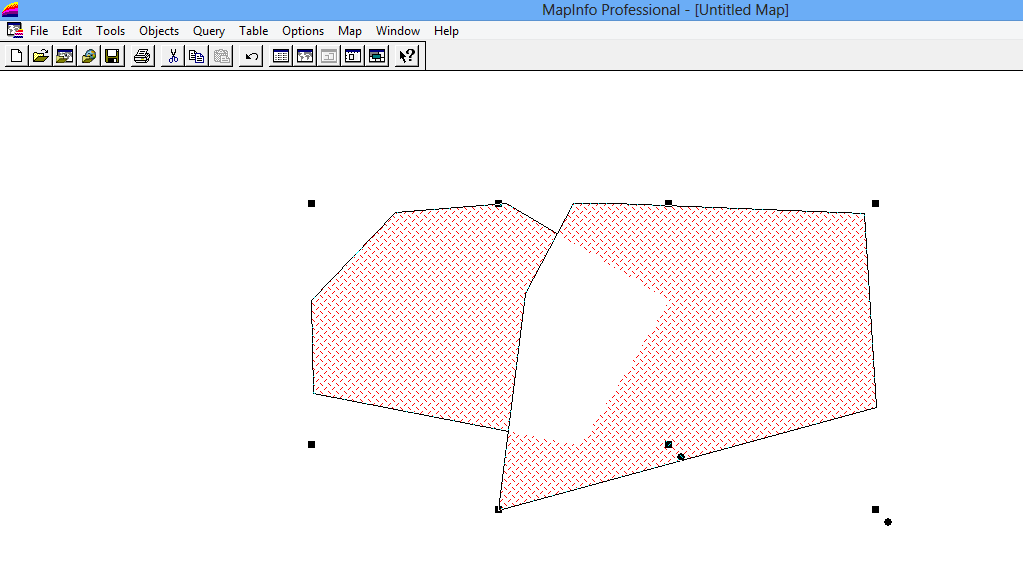
\includegraphics[width=1\textwidth]{./resources/014-dua-objek-untuk-combine}
      \caption{Contoh Bidang-Bidang Berhimpit yang Akan Digabung}
    \end{figure}
    
    Sebagai tambahan bahwa kedua bidang tersebut saling tumpang tindih, sehingga bagian bidang yang saling tumpang tindih tidak terlihat terarsir.
    
    \item Pada menu utama pilih Object -\textgreater Combine atau cukup dengan meng-klik kanan lalu pilih Combine, sehingga akan muncul jendela berikut :
    
    \begin{figure}[H]
      \centering
      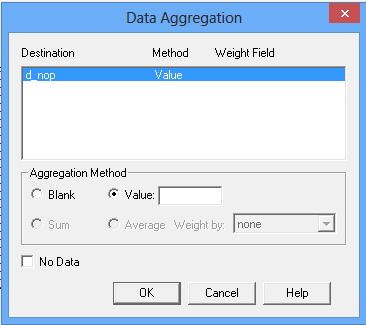
\includegraphics[width=1\textwidth]{./resources/015-window-aggregation-untuk-combine}
      \caption{Jendela Agregasi Data}
    \end{figure}
    
    Karena kedua bidang biasanya memiliki informasi atribut masing-masing, maka diperlukan kejelasan untuk penggabungan datanya pula, melalui jendela inilah kita memberikan informasi atribut untuk objek baru hasil penggabungan.
    
    \item Setelah mengisikan informasi untuk penggabungan/agregasi datanya, jika kita menekan tombol \textbf{Enter} maka kedua objek yang digabung akan terlihat seperti gambar berikut :
    
    \begin{figure}[H]
      \centering
      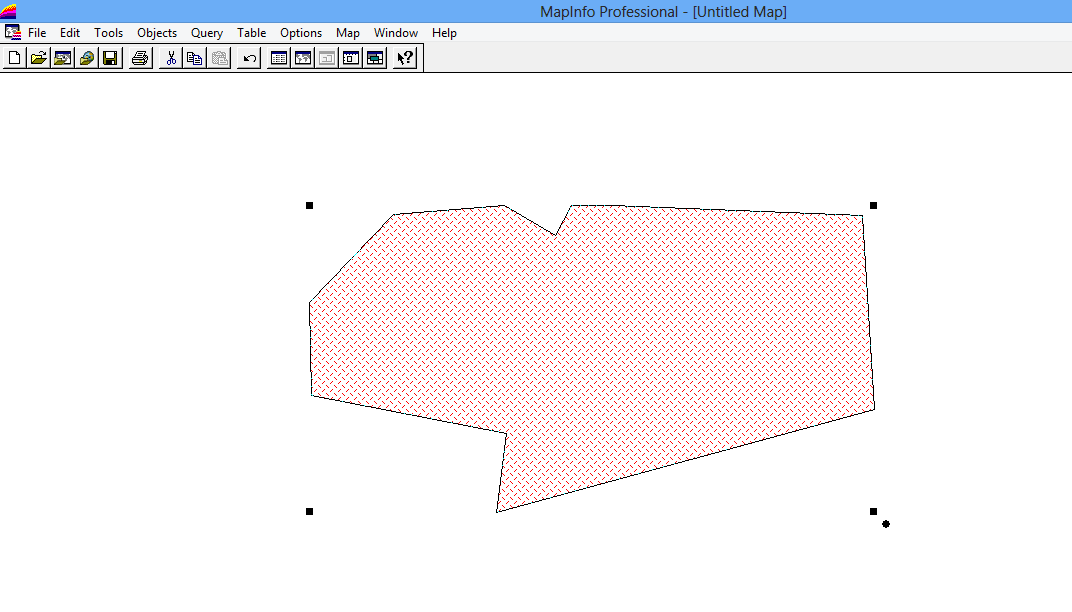
\includegraphics[width=1\textwidth]{./resources/016-objek-hasil-combine}
      \caption{Hasil Penggabungan Kedua Objek}
    \end{figure}
  \end{enumerate}
  
  \item \textbf{Operasi Pemisahan (Split)}
  
  \begin{enumerate}[1.]
    \item Buka layer objek yang akan dilakukan operasi pemisahan, atau membuat layer baru untuk objek yang akan dipisah. Sebagai contoh seperti gambar dibawah ini :
    
    \begin{figure}[H]
      \centering
      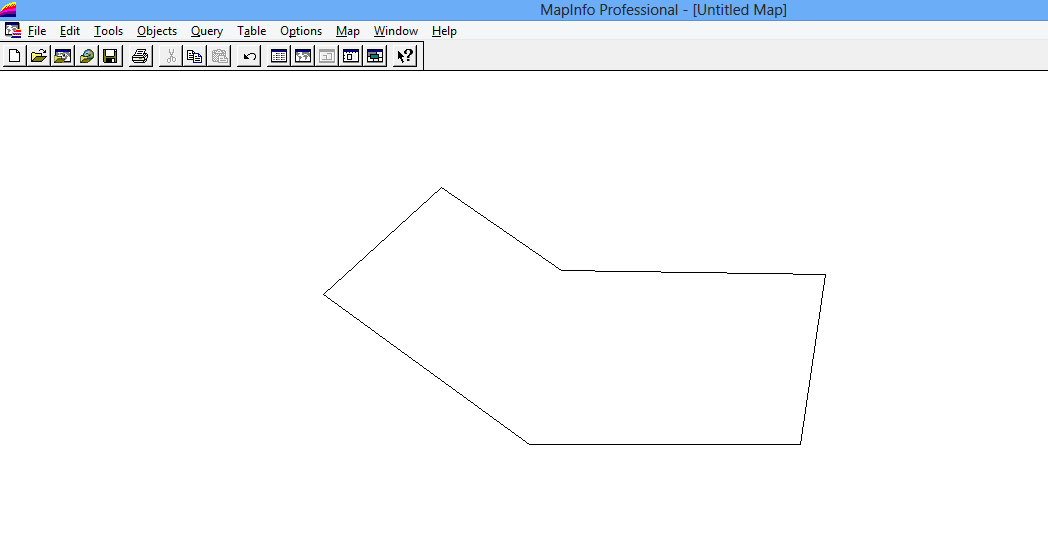
\includegraphics[width=1\textwidth]{./resources/017-layer-untuk-split}
      \caption{Objek yang akan dipisah / split}
    \end{figure}
  
    \item Pilih objek yang akan dipisah menggunakan ikon 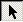
\includegraphics{./resources/008-ikon-select} sehingga objek akan terlihat seperti ini :
    
    \begin{figure}[H]
      \centering
      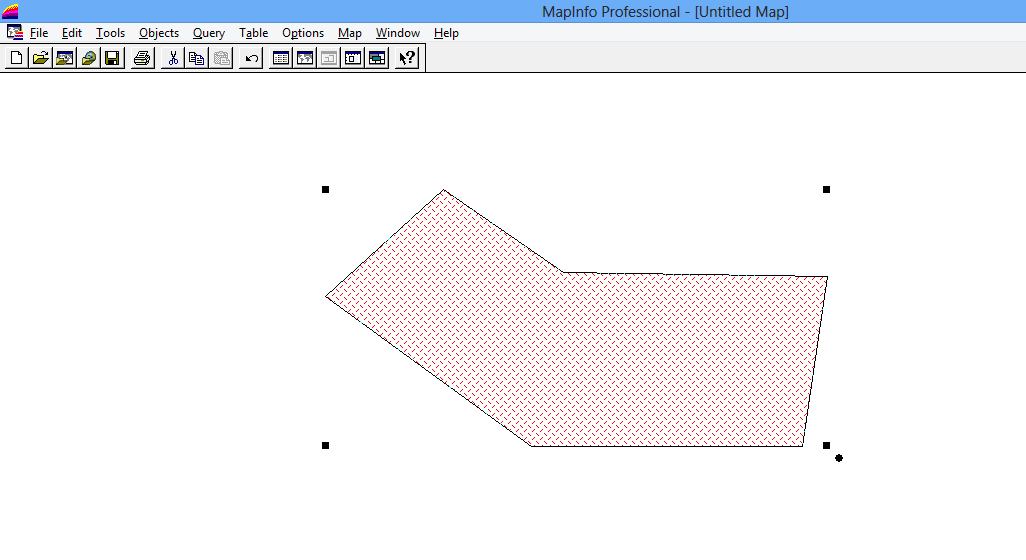
\includegraphics[width=1\textwidth]{./resources/018-objek-terpilih-untuk-split}
      \caption{Objek Yang Dipilih untuk Dipisah/Split}
    \end{figure} 
    
    \item Pilih menu Objects -\textgreater Set Target, sehingga objek menjadi terlihat seperti ini :
    
    \begin{figure}[H]
      \centering
      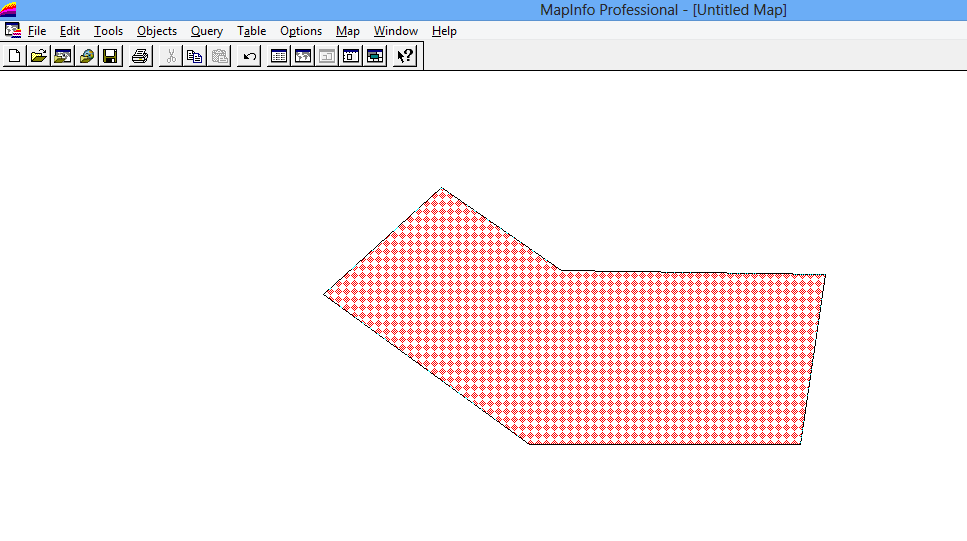
\includegraphics[width=1\textwidth]{./resources/019-objek-terpilih-set-target}
      \caption{Objek Telah Dijadikan Target Split/Pemisahan}
    \end{figure}
    
    \item Buatkan bidang poligon bantu sebagai batas pemisahan objek yang menjadi target, misalkan bidang target akan kita pisah/split menjadi 2 (dua) bagian seperti gambar berikut :
    
    \begin{figure}[H]
      \centering
      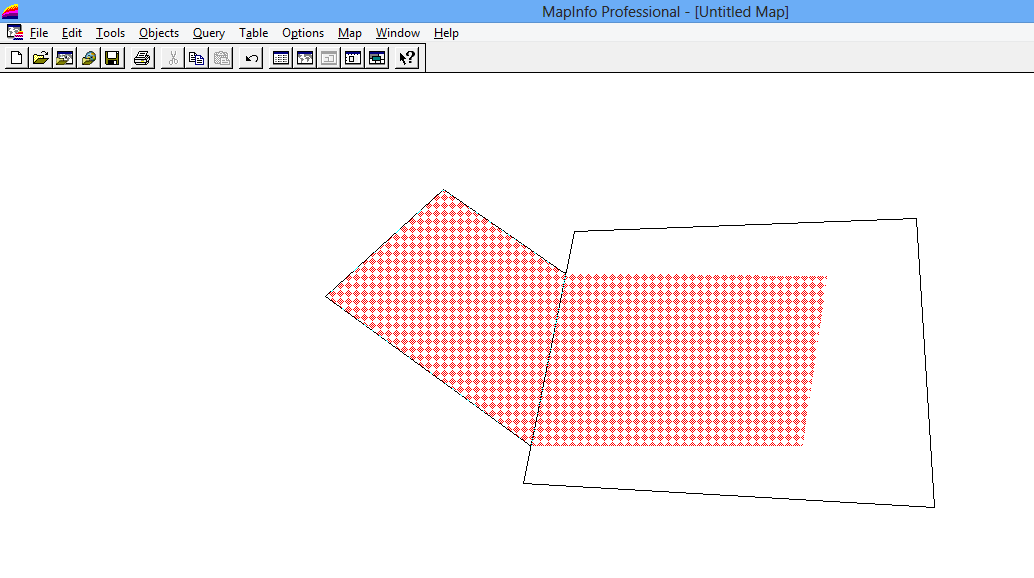
\includegraphics[width=1\textwidth]{./resources/020-poligon-pembantu-split}
      \caption{Objek Poligon Pembantu Untuk Memisahkan/Split Objek Target}
    \end{figure}
    
    \item Pilihlah objek poligon pembantu dengan ikon 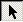
\includegraphics{./resources/008-ikon-select} sehingga objek poligon pembantu menjadi terarsir seperti ini :
    
    \begin{figure}[H]
      \centering
      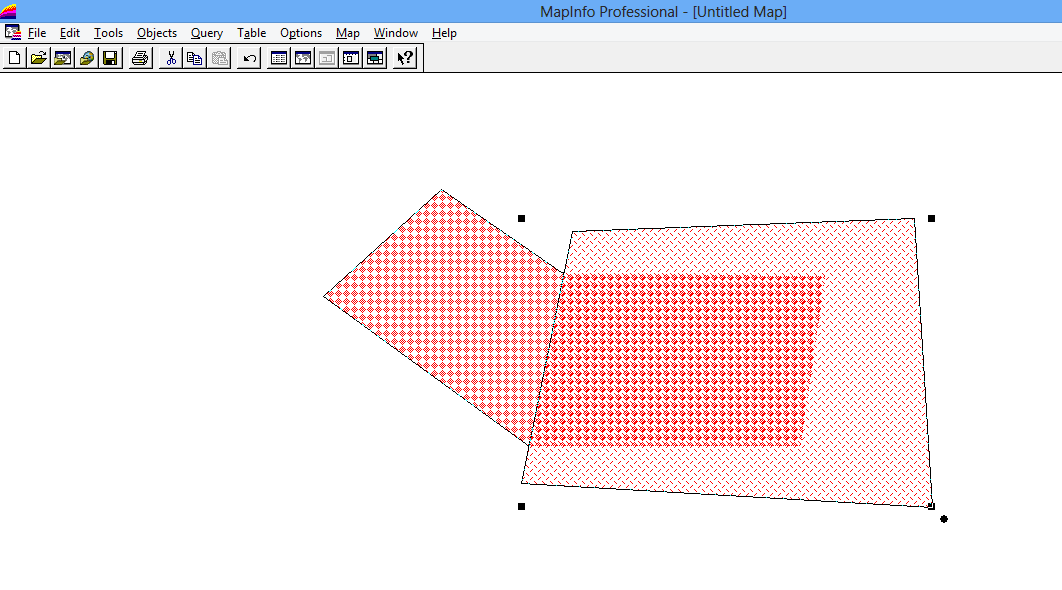
\includegraphics[width=1\textwidth]{./resources/021-poligon-pembantu-terpilih-split}
      \caption{Objek Poligon Pembantu Terpilih}
    \end{figure}
    
    \item Memilih menu Objects -\textgreater Split... sehingga muncul jendela agregasi berikut :
    
    \begin{figure}[H]
      \centering
      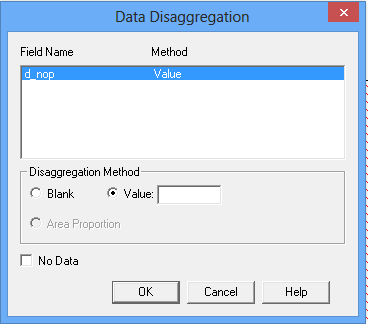
\includegraphics[width=1\textwidth]{./resources/022-window-aggregation-untuk-split}
      \caption{Jendela Aggregation Untuk Pemisahan/Split Objek}
    \end{figure}
    
    Isikan dengan data atribut baru untuk objek yang dipisah/split.
    
    \item Pilih objek poligon pembantu dengan ikon select seperti ini 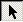
\includegraphics{./resources/008-ikon-select}, kemudian tekan tombol \textbf{delete} pada \textit{keyboard}, sehingga hasil akhir akan terlihat seperti ini :
    
    \begin{figure}[H]
      \centering
      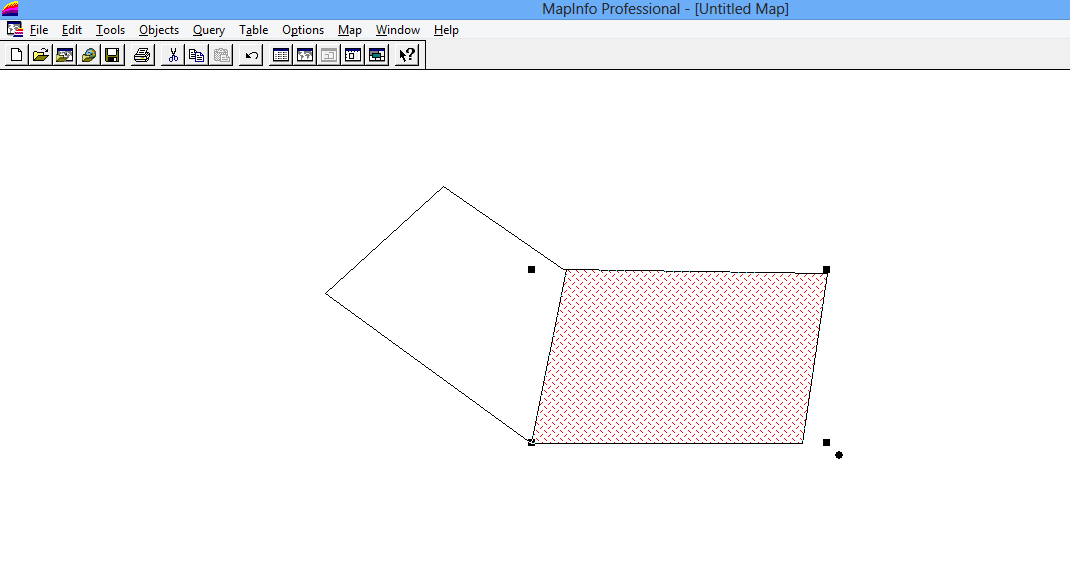
\includegraphics[width=1\textwidth]{./resources/023-objek-hasil-split}
      \caption{Hasil Akhir Operasi Pemisahan/Split}
    \end{figure}
  \end{enumerate}
  
  \item \textbf{Operasi Pemotongan 1 (Erase)}
  
  \begin{enumerate}[1.]
    \item Buka layer yang objeknya akan dilakukan pemotongan, atau buat layer baru dan gambarkan objek yang akan dilakukan operasi pemotongan 1, atau operasi pemotongan didalam. Berikut adalah contohnya :
    
    \begin{figure}[H]
      \centering
      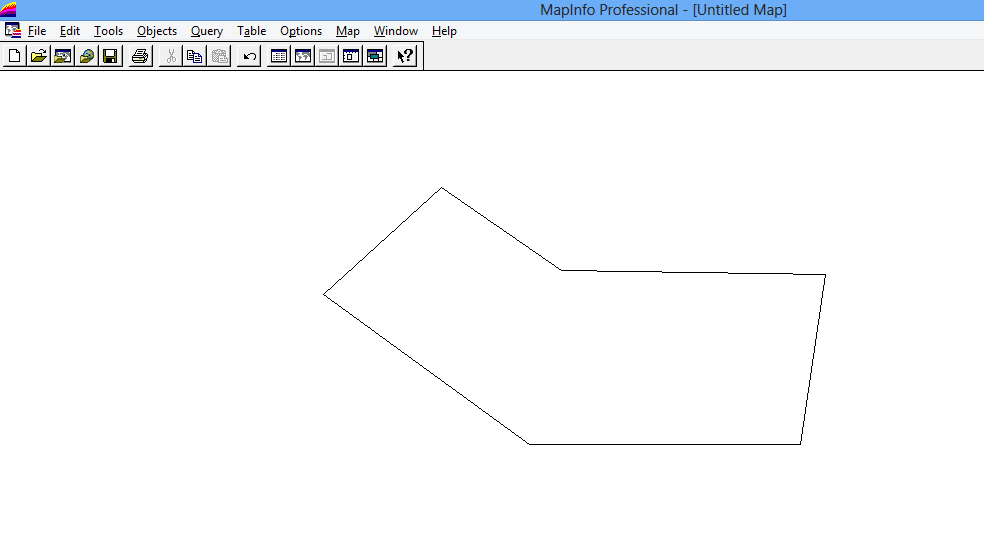
\includegraphics[width=1\textwidth]{./resources/024-layer-untuk-erase}
      \caption{Objek Yang Akan Dilakukan Pemotongan}
    \end{figure}  
  
    \item Pilih objek yang akan di potong menggunakan ikon 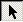
\includegraphics{./resources/008-ikon-select} sehingga akan terlihat seperti berikut :
    
    \begin{figure}[H]
      \centering
      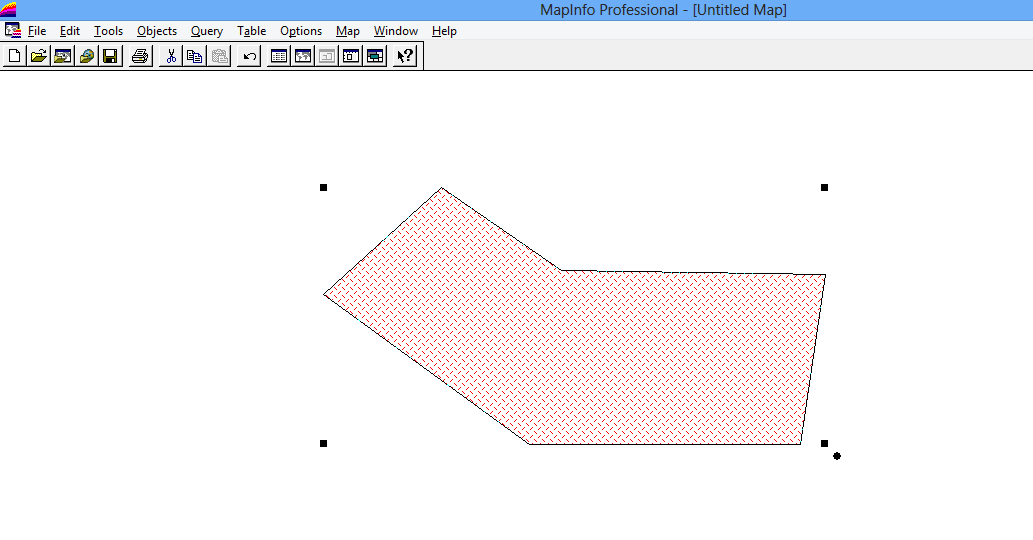
\includegraphics[width=1\textwidth]{./resources/025-objek-terpilih-untuk-erase}
      \caption{Objek Terpilih Untuk Dilakukan Operasi Penghapusan}
    \end{figure}
    
    \item Pilih menu Objects -\textgreater Set Target, sehingga objek terpilih menjadi terlihat seperti ini :
    
    \begin{figure}[H]
      \centering
      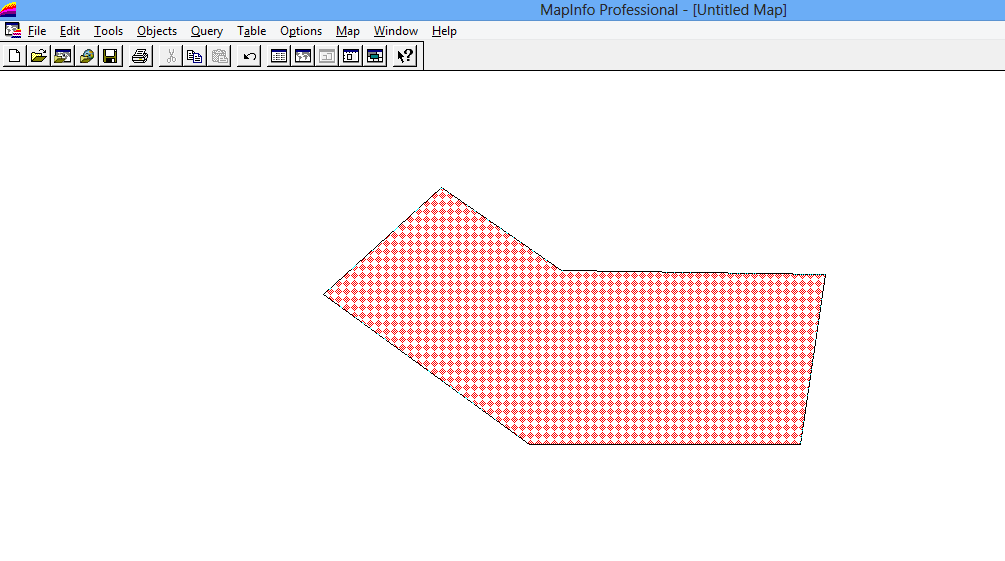
\includegraphics[width=1\textwidth]{./resources/026-objek-tertarget-untuk-erase}
      \caption{Objek Terpilih Sudah Menjadi Target Pemotongan}
    \end{figure}
    
    \item Buat polygon sebagai objek bantu untuk melakukan pemotongan, sebagai contoh seperti gambar berikut :
    
    \begin{figure}[H]
      \centering
      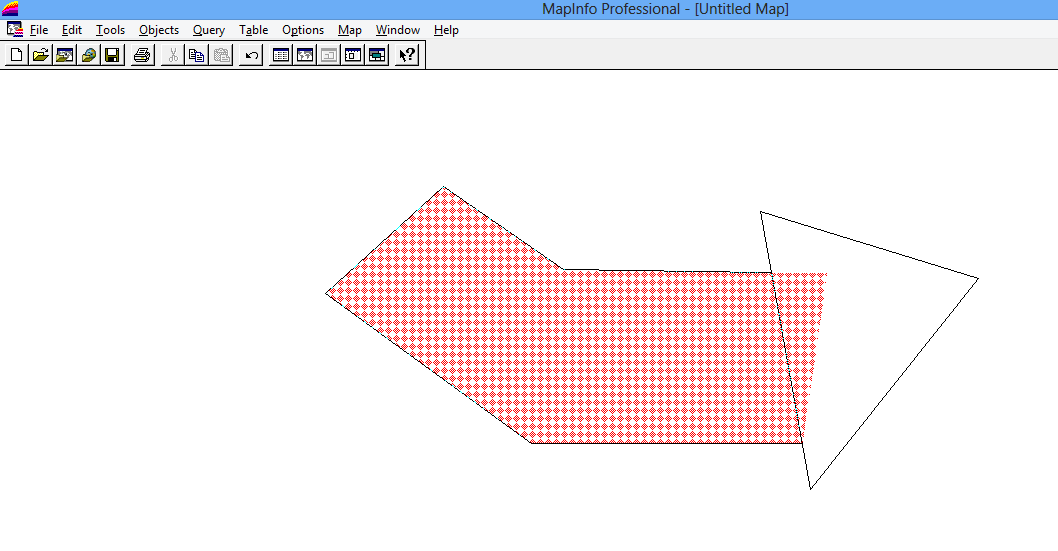
\includegraphics[width=1\textwidth]{./resources/027-objek-pembantu-erase}
      \caption{Objek Pembantu Untuk Melakukan Pemotongan}
    \end{figure}
    
    \item Pilih objek pembantu dengan menggunakan ikon select seperti ini 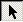
\includegraphics{./resources/008-ikon-select}, sehingga objek pembantu akan terlihat seperti ini :
    
    \begin{figure}[H]
      \centering
      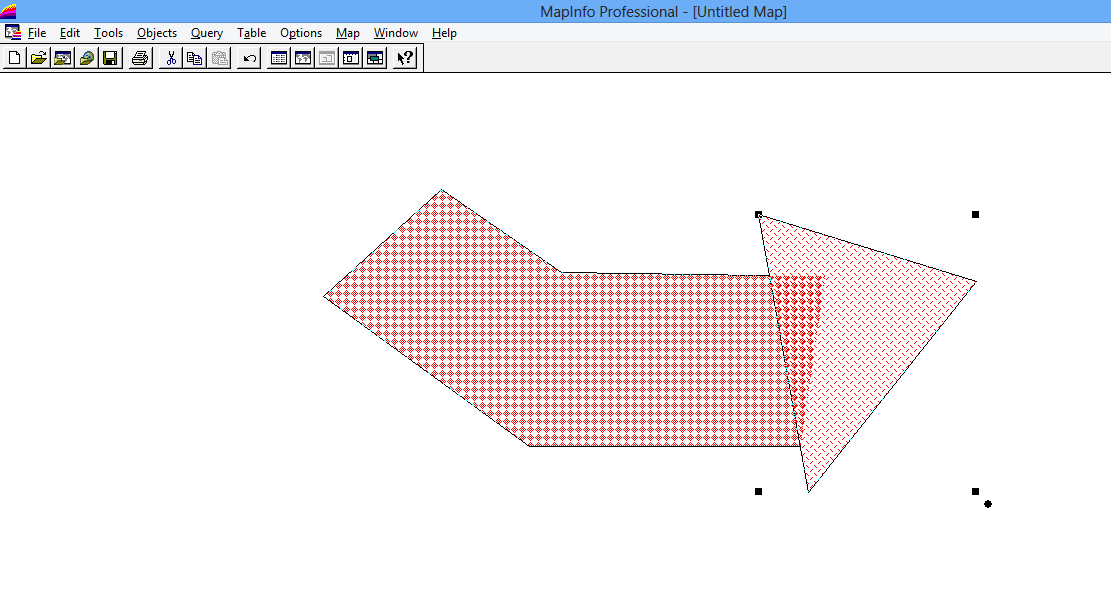
\includegraphics[width=1\textwidth]{./resources/028-objek-pembantu-erase-terpilih}
      \caption{Objek Pembantu Terpilih}
    \end{figure}
    
    \item Pilih menu Objects -\textgreater Erase untuk menghapus bagian yang ada di dalam objek pembantu. Nantinya akan muncul jendela Aggregation seperti ini :
    
    \begin{figure}[H]
      \centering
      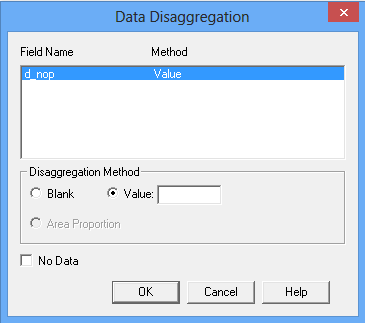
\includegraphics[width=1\textwidth]{./resources/029-window-aggregation-untuk-erase}
      \caption{Jendela Aggregation Untuk Objek Yang Tersisa}
    \end{figure}
    
    \item Setelah menekan tombol \textbf{OK} pada jendela Aggregation, maka objek sebenarnya sudah terpisah, seperti gambar berikut ini contohnya :
    
    \begin{figure}[H]
      \centering
      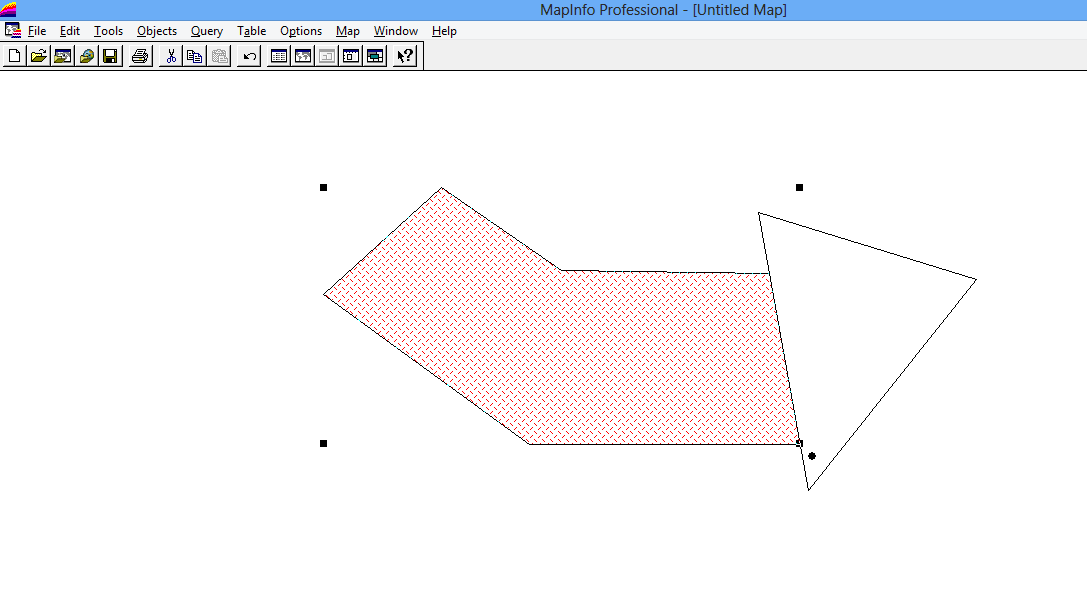
\includegraphics[width=1\textwidth]{./resources/030-objek-telah-terpotong}
      \caption{Objek Telah Terpotong}
    \end{figure}
    
    \item Hapus objek pembantu dengan ikon select 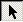
\includegraphics{./resources/008-ikon-select}, kemudian memilih objek pembantu tersebut dan menekan tombol \textbf{delete} pada \textit{keyboard}, sehingga akan didapat hasil akhir berikut :
    
    \begin{figure}[H]
      \centering
      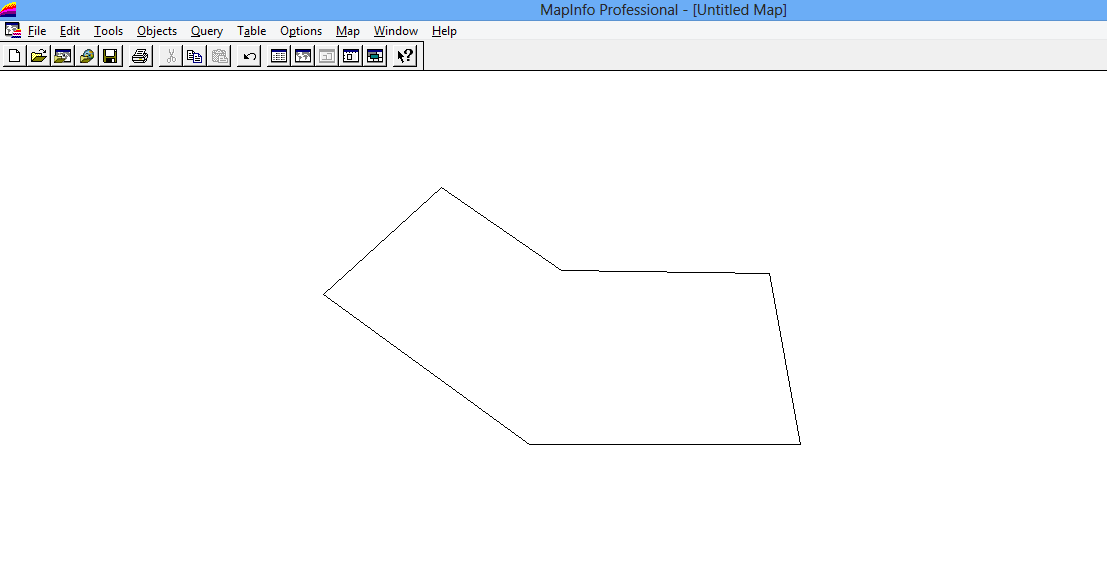
\includegraphics[width=1\textwidth]{./resources/031-hasil-akhir-erase}
      \caption{Hasil Akhir Pemotongan}
    \end{figure}
  \end{enumerate}
  
  \item \textbf{Operasi Pemotongan 2 (Erase Outside)}
  
  \begin{enumerate}[1.]
    \item Buka terlebih dahulu layer yang objeknya akan dipotong, atau buat layer baru dan buatkan objek yang akan dilakukan operasi pemotongan. Sebagai contoh seperti gambar berikut :
    
    \begin{figure}[H]
      \centering
      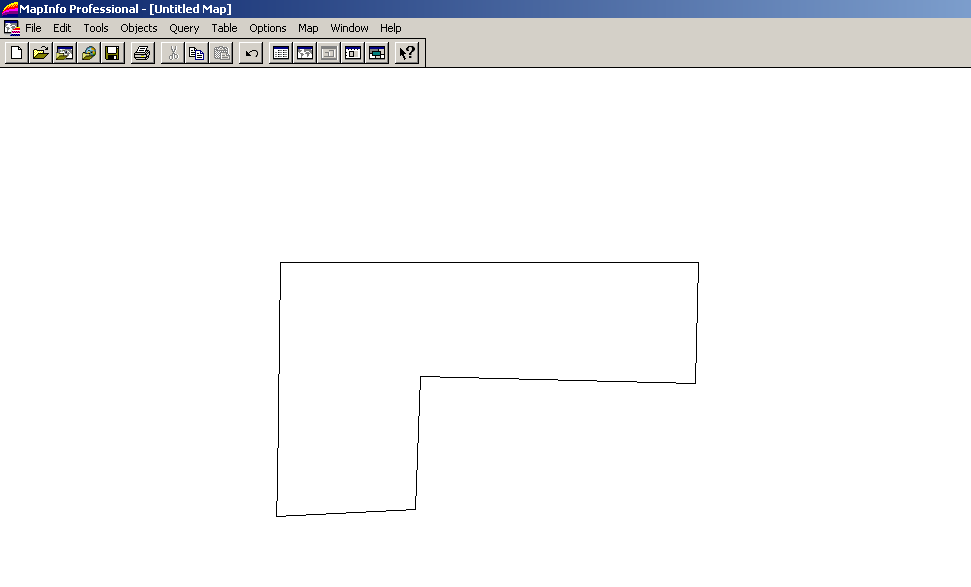
\includegraphics[width=1\textwidth]{./resources/032-layer-untuk-erase-2}
      \caption{Layer Objek Yang Akan Dipotong}
    \end{figure}
  
    \item Pilih objek yang akan di potong dengan menggunakan ikon 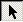
\includegraphics{./resources/008-ikon-select} sehingga objek akan terlihat seperti ini :
    
    \begin{figure}[H]
      \centering
      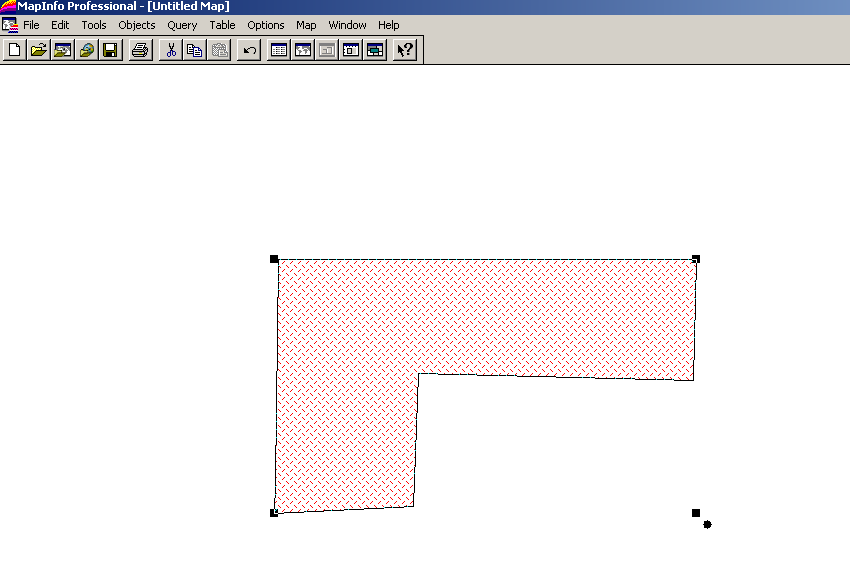
\includegraphics[width=1\textwidth]{./resources/033-objek-terpilih-untuk-erase-2}
      \caption{Objek Yang Terpilih Untuk Dilakukan Pemotongan}
    \end{figure}
    
    \item Pilih menu Objects -\textgreater Set Target sehingga objek yang akan dipotong terlihat seperti ini :
    
    \begin{figure}[H]
      \centering
      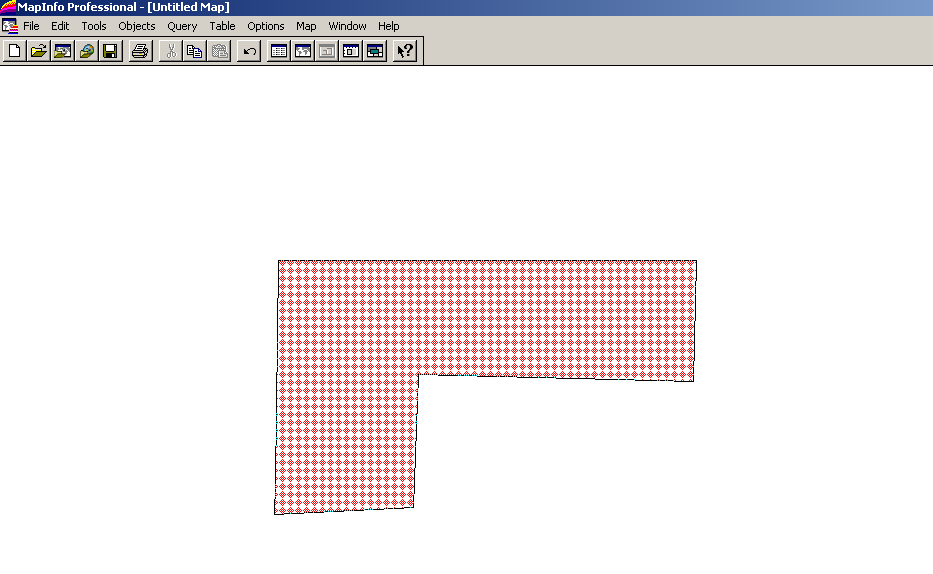
\includegraphics[width=1\textwidth]{./resources/034-objek-tertarget-untuk-erase-2}
      \caption{Objek Tertarget Untuk Dilakukan Pemotongan}
    \end{figure}
    
    \item Buat objek poligon bantuan untuk melakukan pemotongan objek, nantinya objek diluar poligon bantuan ini akan terhapus, sebagai contoh seperti gambar berikut :
    
    \begin{figure}[H]
      \centering
      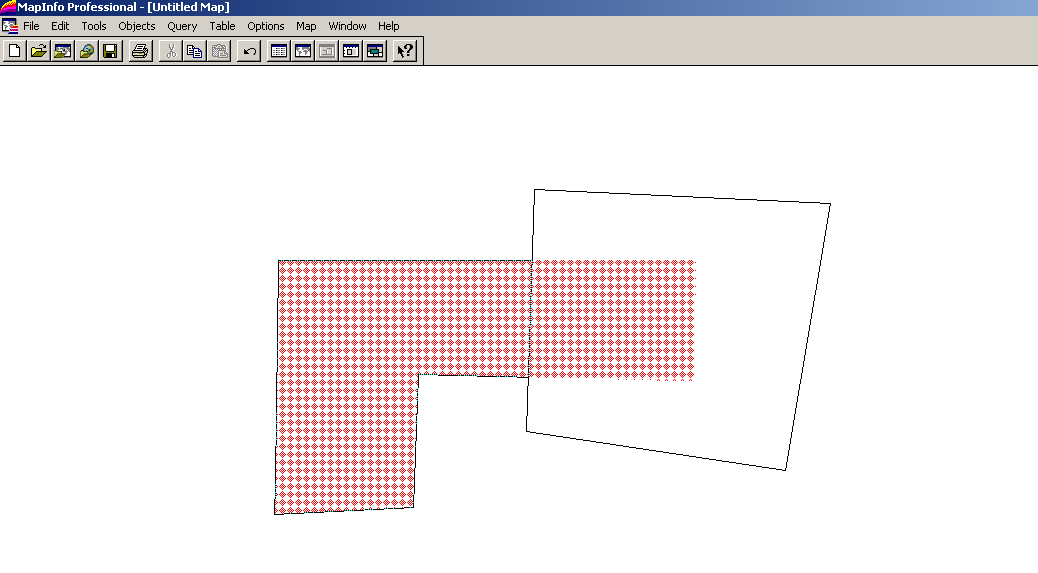
\includegraphics[width=1\textwidth]{./resources/035-poligon-bantuan-untuk-erase-2}
      \caption{Objek Poligon Bantuan Untuk Melakukan Pemotongan}
    \end{figure}
    
    \item Pilih objek poligon bantuan dengan menggunakan ikon 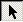
\includegraphics{./resources/008-ikon-select}, sehingga objek tersebut akan terlihat seperti ini :
    
    \begin{figure}[H]
      \centering
      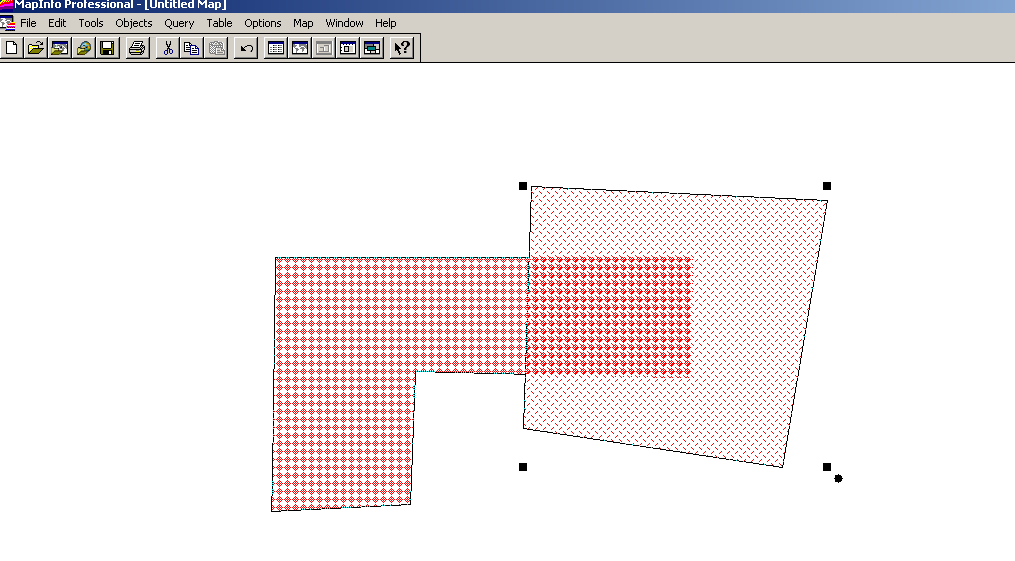
\includegraphics[width=1\textwidth]{./resources/036-poligon-bantuan-terpilih-untuk-erase-2}
      \caption{Objek Poligon Bantuan Terpilih}
    \end{figure}
    
    \item Memilih menu Objects -\textgreater Erase Outside..., sehingga muncul jendela aggregate seperti ini :
    
    \begin{figure}[H]
      \centering
      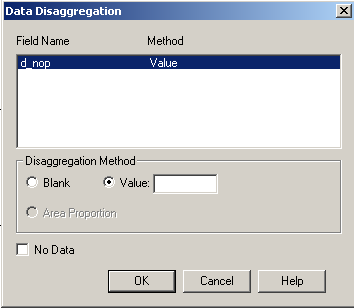
\includegraphics[width=1\textwidth]{./resources/037-jendela-aggregate-untuk-erase-2}
      \caption{Jendela Aggregate Untuk Pemotongan}
    \end{figure}
    
    Isiannya adalah berupa atribut data untuk objek yang nantinya masih tersisa.
    
    \item Setelah dilakukan pengisian atribut data untuk objek yang terpisah, hasilnya akan terlihat seperti gambar berikut :
    
    \begin{figure}[H]
      \centering
      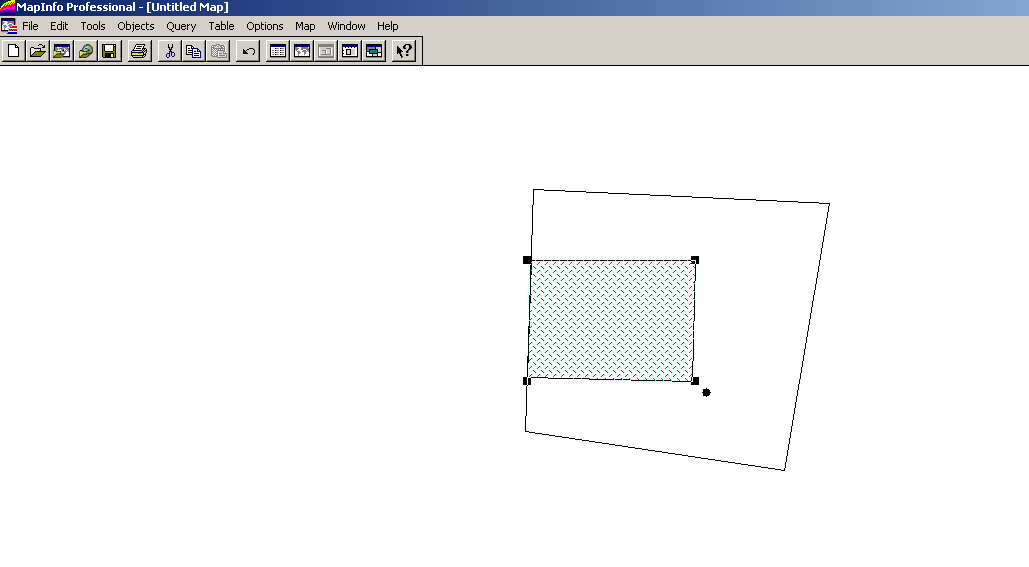
\includegraphics[width=1\textwidth]{./resources/038-objek-target-terpotong-erase-2}
      \caption{Objek Yang Masih Tersisa Dari Hasil Pemotongan}
    \end{figure}
    
    \item Pilih objek poligon bantuan dengan menggunakan ikon 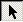
\includegraphics{./resources/008-ikon-select}, kemudian tekan tombol \textbf{delete} pada \textit{keyboard}, sehingga menghasilkan objek seperti gambar di bawah ini :
    
    \begin{figure}[H]
      \centering
      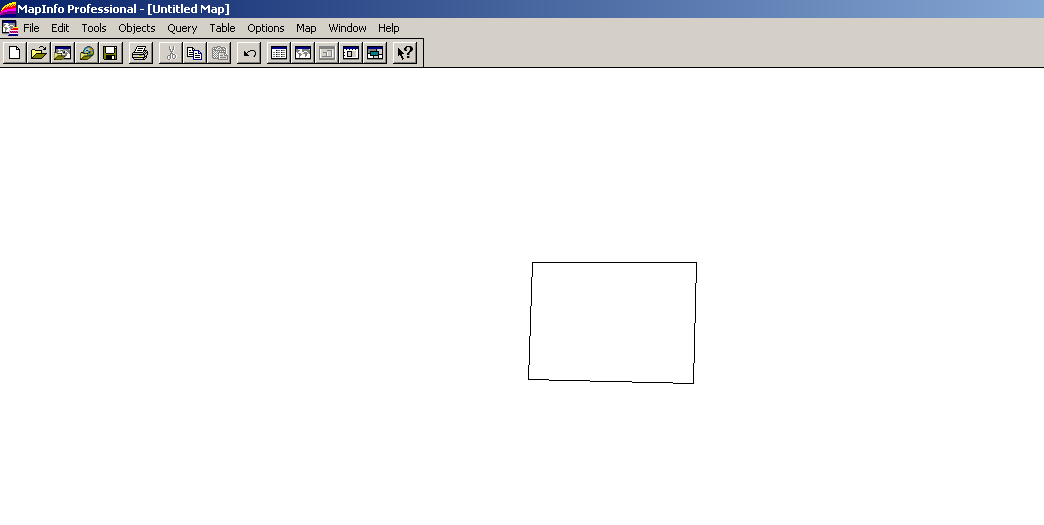
\includegraphics[width=1\textwidth]{./resources/039-hasil-erase-2}
      \caption{Hasil Akhir Pemotongan}
    \end{figure}
  \end{enumerate}
  
  \item \textbf{Menyambung Vertex (Snap)}
  
  \begin{enumerate}[1.]
    \item Buka layer yang objeknya saling terpisah atau bertumpukan kemudian akan disambungkan / dihimpitkan, atau sebagai contoh dapat membuat layer baru untuk hal ini seperti contoh gambar berikut :
    
    \begin{figure}[H]
      \centering
      \includegraphics[width=1\textwidth]{./resources/040-layer-sambung-vertex}
      \caption{Contoh Dua Objek Yang Akan Disambungkan}
    \end{figure}
    
    \item Pilih objek yang akan disambung dengan menggunakan ikon select \includegraphics{./resources/008-ikon-select}, sehingga objek akan terlihat seperti gambar berikut :
    
    \begin{figure}[H]
      \centering
      \includegraphics[width=1\textwidth]{./resources/041-objek-reshape-terpilih}
      \caption{Objek Yang Terpilih Untuk Dilakukan Reshape Penyambungan}
    \end{figure}
    
    \item Tekan huruf S pada \textit{keyboard}. Perhatikan tanda Snap yang muncul di bagian bawah jendela MapInfo yang menandakan, berarti Snap aktif. Untuk menonaktifkan Snap, tekan S kembali. Aktifnya fungsinya snap ini ditandai seperti gambar berikut :
    
    \begin{figure}[H]
      \centering
      \includegraphics[width=1\textwidth]{./resources/042-snap-aktif}
      \caption{Tanda Tombol Snap Aktif}
    \end{figure}
    
    \item Pilih ikon \textit{reshape} \includegraphics{./resources/043-ikon-reshape}, dan pindahkan titik-titik objek agar berhimpit/menyambung seperti gambar berikut :
    
    \begin{figure}[H]
      \centering
      \includegraphics[width=1\textwidth]{./resources/044-reshape-snap-ke-objek-lain}
      \caption{Hasil Reshape Objek}
    \end{figure}
  \end{enumerate}

\end{enumerate} 